\documentclass[12pt,answers]{exam}
\usepackage[a4paper,
            left=1in,
            right=1in,
            top=1in,
            bottom=1in,
            footskip=.25in]{geometry}
\usepackage{tikz}
\usetikzlibrary{calc, through,intersections}
\usepackage{xparse}
\usepackage{caption}
\usepackage{amssymb}
\usepackage{physics}
\date{\today}
\renewcommand{\thequestion}{\textbf{Problem \arabic{question}}}
\unframedsolutions
\begin{document}
\title{Maths Circle Challenge}
% \author{Maths Circle India}
\maketitle
\thispagestyle{empty}
\section*{Dividing a Field}

\begin{questions}
\question A farmer's field is irregularly shaped, as shown in the figure. The terrain is flat and the boundary lines are all in the North-South or East-West direction. The farmer has two sons and wants to divide the land into two pieces of land with equal area. He has before him a map of the land and an old school geometry box. The box has a compass and a ruler, whose markings are faded and unreadable. Can you help the farmer divide the land with the instruments he has?
\begin{figure}[h]
    \centering
    \begin{tikzpicture}[scale=0.7]
        \draw[thick] (0,0) -- (5,0) -- (5,5) -- (8,5) -- (8,10) -- (0,10) -- cycle;
        \draw[thick,->] (0,11) --+(0,1) node[left] {$N$};
        \draw[thick,->] (9,11) --+(1,0) node[below] {$E$};
    \end{tikzpicture}
    \caption{Figure shows an irregular piece of land owned by the Farmer. The problem is to divide the land into two pieces of equal area using only a straight edge and compass.}
\end{figure}
\begin{solution}
    A line through the centre of the rectangle divides it into two equal areas.
    \begin{itemize}
        \item[Step 1:] Find the $O_a$ centre of the extended rectangle $ABCD$.
        \item[Step 2:] Find the centre of the missing rectangle portion, call it $O_b$.
        \item[Step 3:] Connect $O_a$ and $O_b$.
    \end{itemize}
        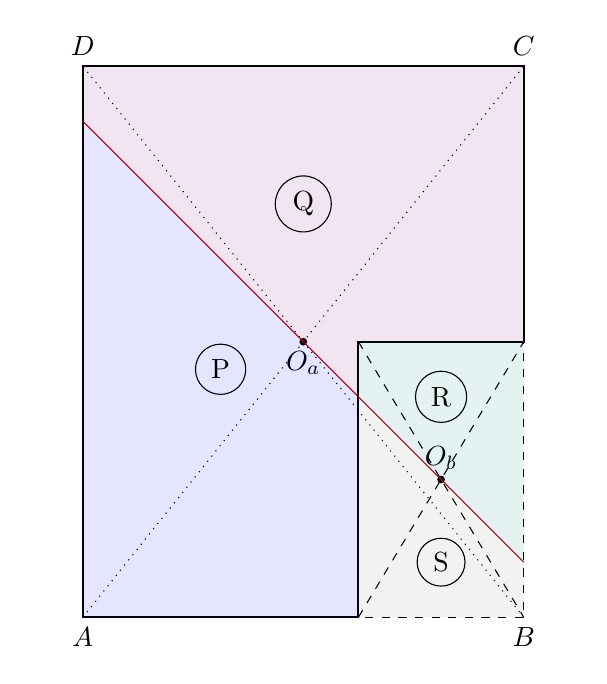
\begin{tikzpicture}[scale=0.7]
            \draw[thick] (0,0) coordinate (A) node[below] {$A$} -- (5,0) coordinate (P) -- (5,5) coordinate (Q) -- (8,5) coordinate (R) -- (8,10) coordinate (C) node[above] {$C$} -- (0,10) coordinate (D) node[above] {$D$} -- cycle;
            \draw[dashed] (A) rectangle (C);
            \draw (8,0) coordinate (B) node[below] {$B$};
            \draw[dotted, name path=diag R1] (A) -- (C);
            \draw[dotted, name path=diag R2] (B) -- (D);
            \fill [name intersections={of=diag R1 and diag R2, by={a}}] (a) node[below] {$O_a$} circle (2pt);
            \draw[dashed, name path=diag r1] (P)-- (R);
            \draw[dashed, name path=diag r2] (Q)-- (B);
            \fill [name intersections={of=diag r1 and diag r2, by={b}}] (b) node[above] {$O_b$} circle (2pt);
            
            \path[name path=line_ab] ($(a)!-2!(b)$) -- ($(a)!2!(b)$);
            \path[name path=line_AD] (A) -- (D);
            \path[name path=line_BC] (B) -- (C);

            \path [name intersections={of=line_ab and line_AD, by={left_inter}}];
            \path [name intersections={of=line_ab and line_BC, by={right_inter}}];

            \draw[red!70!black] (left_inter) -- (right_inter);

            \path [name path=line_PQ] (P) -- (Q);
            \path [name intersections={of=line_ab and line_PQ, by={small_left}}];

            \fill[blue,opacity=0.1] (P) -- (A) -- (left_inter) -- (small_left) -- cycle;
            \node[circle, draw, inner sep=3pt] at ($(left_inter)!0.5!(P)$) {P};

            \fill[blue!50!red,opacity=0.1] (small_left) -- (left_inter) -- (D) -- (C) -- (R) -- (Q) -- cycle;
            \node[circle, draw, inner sep=3pt] at ($(D)!0.5!(R)$) {Q};

            \fill[blue!50!green,opacity=0.1] (small_left) -- (right_inter) -- (R) -- (Q) -- cycle;
            \node[circle, draw, inner sep=3pt] at ($(Q)!0.5!(right_inter)+(0,1)$) {R};

            \fill[blue!50!yellow,opacity=0.1] (small_left) -- (right_inter) -- (B) -- (P) -- cycle;
            \node[circle, draw, inner sep=3pt] at ($(B)!0.5!(small_left)+(0,-1)$) {S};
        \end{tikzpicture}
    \captionof{figure}{The line through $O_a$ and $O_b$ divides the extended rectangle into four regions - P, Q, R, and S.}
    \[\begin{aligned}
    &P+S = Q+R,\\
    &S = R,\\
    &\text{and therefore } P = Q    
    \end{aligned}\]
\end{solution}
\question Prove that for any integer $n$, $n^3+11n$ is a multiple of 6.
\begin{solution}
\[    \begin{aligned}
        \text{Case 1a: } &n \equiv 0 \pmod{2}, n \text{ is even}\\
        &\text{then } n^3+11n \equiv 0 \pmod{2}\\        
        \text{Case 1b: }&n \equiv 1 \pmod{2},\ n \text{ is odd}\\
        &\text{then } n^3 \equiv 1 \pmod{2} \text{ and } 11n \equiv 1 \pmod{2}\\
        &\text{so } n^3 + 11n \equiv 0 \pmod{2}\\
        &n^3+11n \text{ is divisible by 2 for all }n.\\
        \text{Case 2a: } &n \equiv 0 \pmod{3}\\
        &\text{then } n^3+11n \equiv 0 \pmod{3}\\
        \text{Case 2b: } &n \equiv 1 \pmod{3},\ n=3x+1\\
        &n^3+11n = 12 + 42 x + 27 x^2 + 27 x^3 = 3\times(4 + 14 x + 9 x^2 + 9 x^3) \equiv 0 \pmod{3}\\
        \text{Case 2c: } &n \equiv 2 \pmod{3},\ n=3x+2\\
        &n^3+11n = 30 + 69 x + 54 x^2 + 27 x^3 = 10 + 23 x + 18 x^2 + 9 x^3 \equiv 0 \pmod{3}
    \end{aligned}\]
    Method 2:
    \[\begin{aligned}
        &\text{Let } n^3 + 11n = n(n^2+11) = p\\
        &\text{when } n \text{ is odd}, (n^2+11) \text{ is even, making } p \text{ even.}\\ 
        &\text{when } n \text{ is even}, p \text{ is even.}\\
        &\text{when } n \text{ is a multiple of }3,\ p \text{ is also a multiple of } 3.\\
        &n^2 + 11 = (n+1)(n-1)+12.\\
        &\text{When } n \text{ is not a multiple of } 3, \text{ either } n+1 \text{ or } n-1 \text{ is a multiple of }3.\\
        &\text{This makes }n^2+11 \text{ a multiple of }3 \text{ when } n \text{ is not.}         
    \end{aligned}\]
    Method 3: Proof by induction
    \[
        \begin{aligned}
            &\text{Let } P(n) \text{ be the statement that }n^3+11n \equiv 0 \pmod{6}\\
            &\text{For } n= 1,\ n^3+11n = 12 \equiv 0 \pmod{6}\\
            &P(1) \text{ is correct.}\\
            &\text{Assume } P(k) \text{ is correct}.\\
            &k^3 + 11k \equiv 0 \pmod{6}.\\
            &(k+1)^3 + 11(k+1) = k^3 + 11 k + 12 + 3 k(k+1)\\
            &3 k(k+1) \equiv 0 \pmod{2} \text{ for any } k\\
            &3 k(k+1) \equiv 0 \pmod{3} \text{ for any } k\\
            &(k+1)^3 + 11(k+1) \equiv 0 \pmod{6} \text{ or } P(k+1) \text{ is correct. }
        \end{aligned}\]
        The same proof can be used for \( n < 0,\ n \in \mathbb{Z}\). Let \(n=-m\) where \(m \in \mathbb{Z}^+\). $(-m)^3 + 11(-m) = -(m^3+11m)$. Since \(m^3+11m \equiv 0 \pmod{6}\) for \(m \in \mathbb{Z}^+\), \(-(m^3+11m) \equiv 0 \pmod{6}\).
    
        Method 4:
        \[
            \begin{aligned}
        &n^3+11n = n(n^2 + 11) = n((n+1)(n-1)+12)= (n+1)n(n-1) + 12n\\
        &(n+1)n(n-1) \equiv 0 \pmod{2}\ \forall\ n \in \mathbb{Z}\\
        &\text{and } (n+1)n(n-1) \equiv 0 \pmod{3}\ \forall\ n \in \mathbb{Z}\\
        &\implies (n+1)n(n-1) \equiv 0 \pmod{6}\ \forall\ n \in \mathbb{Z}\\
        &12n \equiv 0 \pmod{6}\ \forall\ n \in \mathbb{Z}\\
        &\implies (n+1)n(n-1) + 12n = n^3+11n \equiv 0 \pmod{6}\ \forall\ n \in \mathbb{Z}
            \end{aligned}
            \]
\end{solution}
\question A couple (let's call them Sharmila and Prakash) invite five couples over for dinner. When they meet, there are introductions and some of the people shake hands. Of course, one does not shakes one's own hand and that of his/her spouse. Sharmila notices that of the other people (excluding herself) in the gathering, no two people shake the same number of hands. How many hands does Prakash shake?
\begin{solution}
    There are 11 people, each engaging in a handshake with some or none of the others. Each person shakes a number of hands from the set \(\{0,1,2,3,4,5,6,7,8,9,10\}\). Let $P_k$ be the person who shook $k$ hands. 
    
    $P_{10}$ shook everyone's hands except their spouse's and $P_{0}$. This accounts for 13 people ($P_{10}$, thier spouse, the 10 people they shake hands with, and $P_{0}$). $P_0$ and $P_{10}$ are a couple. $P_1$ shakes hands only with $P_{10}$. $P_{9}$ has to shake 8 more hands other than that of $P_0,\ P_1,\ P_{10},$ their spouse, or self. The only way to ensure distinct handshakes is for $P_9$ to be the spouse of $P_1$.
    By extending this logic, one can see that $P_{10-n}$ and $P_n$ are a couple for \(n\in\{0,1,2,3,4\}\) and $P_5$ is unpaired. 

    This means that $P_5$ and another person both shook the same number of hands. 
    
    Since no two people shake the same number of hands (excluding Sharmila), but we now have two people shaking 5 hands. Thus, $P_5$ must be Prakash who shakes the same number of hands as his spouse Sharmila.

    Prakash shook hands with 5 people. 
\end{solution}
\question Let us make the following definition. We call any finite sequence of English letters ``a word" (whether or not it can be found in a dictionary). For example, we can form six words using the letters A, B, and C each exactly once: ABC, ACB, BAC, BCA, CAB, and CBA. In the following calculate the number of different words that can be obtained by rearranging the letters of the word.
\begin{parts}
    \part MESOPOTAMIA
    \begin{solution}
        The formula for the number of distinct permutations of a multiset is:
        \[
            \frac{n!}{k_1!k_2!...k_m!}
        \]
        \[
        \frac{11!}{2!2!2!} = 4989600
        \]
    \end{solution}
    \part SCRAMBLE
    \begin{solution}
        \[
        8! = 40320
        \]
    \end{solution}
    \part JUXTAPOSITION
    \begin{solution}
        \[
        \frac{13!}{2!2!2!} = 778377600
        \]
    \end{solution}
    \part VIOLIN
    \begin{solution}
        \[
        \frac{6!}{2!} = 360
        \]
    \end{solution}
    \part MISSISSIPPI
    \begin{solution}
        \[
        \frac{11!}{4!4!2!}=34650
        \]
    \end{solution}
\end{parts}
\question Mr. and Mrs. Sharma have four children - three boys and a girl - who each likes one of the colours - blue, green, red, yellow - and one of the letters - P, Q, R, S. The oldest child likes the letter Q. The youngest child likes green. Aditya likes the letter S. Bhanumati, the girl, has an older brother who likes R. The one who likes blue isn't the oldest. The one who likes red likes the letter P. Chetan likes yellow. Based on the above facts, Deepak is the
\begin{choices}
    \choice youngest child
    \choice third child
    \CorrectChoice second child
    \choice oldest child
\end{choices}
\begin{solution}
    \begin{tabular}{lllll}
        \hline
        1 & Boy	&	yellow	&	Q	&	Chethan	\\\hline
        2 & Boy	&	blue	&	R	&	Deepak	\\\hline
        3 & Girl	&	red	&	P	&	Bhanumati	\\\hline
        4 & Boy	&	green	&	S	&	Aditya	\\\hline
      \end{tabular}
\end{solution}
\question When we throw a die, the numbers one to six are all equally likely. When we throw a pair of dice, the ``outcome" of the throw is usually defined as the sum of the two numbers appearing on top of the dice. Let us change the rules and define the ``outcome" as the product of the two numbers.

How many distinct outcomes are there? What is the chance (probability) that the outcome is

\begin{parts}
    \part a prime number
    \begin{solution}
        \[
            \text{There are 18 distinct outcomes} = \{1,2,3,4,5,6,8,9,10,12,15,16,18,20,24,25,30,36\}
            \]
        The outcomes with prime numbers are \(\{(1,2),(2,1),(1,3),(3,1),(1,5),(5,1)\}\).

        P(prime)= \(\flatfrac{6}{36} = \flatfrac{1}{6}\)   
    \end{solution}
    \part a perfect square
    \begin{solution}
    Favourable outcomes are \(\{(1,1),(2,2),(3,3),(1,4),(4,1),(4,4),(5,5),(6,6)\}\).
    P\(=\flatfrac{8}{36}=\flatfrac{2}{9}\).
    \end{solution}
    \part a triangular number
    \begin{solution}
    Triangular numbers are of the form \(\flatfrac{n(n+1)}{2}\). Favourable outcomes are \(\{(1,1), (1,3),(3,1), (3,2),(2,3), (2,5),(5,2), (5,3),(3,5), (6,6)\}\).
    
    P \(=\flatfrac{10}{36} = \flatfrac{5}{18}\).
\end{solution}
    \part an even number
    \begin{solution}
    P(even) = 1 - P(odd). Odd numbers happen when outcomes are of the form (odd, odd). There 9 (odd,odd) outcomes.

    P \(1 - \flatfrac{9}{36} = \flatfrac{3}{4}\)
    \end{solution}
    \part an odd number
    \begin{solution}
        From previous answer
    P = \(\flatfrac{1}{4}\)
    \end{solution}
    \part both triangular and square
    \begin{solution}
        The only triangular number that is also a square is 1. \(\{(1,1), (6,6)\}\) is the favourable outcome.
        
        P \(=\flatfrac{2}{36} = \flatfrac{1}{18}\).
    \end{solution}
\end{parts}
\question $10$ cables were laid across the Zambezi river in a remote part of Africa. After laying the cables, the engineer realised that he had forgotten to label them, so he didn't know which of the $10$ ends on one bank corresponded to the $10$ ends on the other. He had at his disposal a multimeter to test continuity, some copper wire to connect the ends on each bank and a boat to cross the river with.  As you may know, the Zambezi river has herds of hippos and these  animals can be dangerous to crossing boats. It would be wise to minimise the number of river crossings.

How would the engineer figure out the corresponding cables with a minimum number of crossings?
\end{questions}
\end{document}

